\chapter{Background}
This chapter introduces the necessary background information needed for understanding the rest of the report.
First section, provides a broad introduction to \ac{sdr} systems, GNU Radio Software Tool and \ac{PHY} and \ac{mac} layers of the network stack.
Then the problems mentioned earlier are conceptualized theoretically.
The second section introduces previous work in this domain, which are critically analyzed to help concretely define the problem area.
Finally the last section, introduces the LimeSDR platform, IEEE 802.15.4 based system design and the tools used in the methods section.


\section{Essential Concepts}
\subsection{\ac{PHY} and \ac{mac} Layers}
\ac{OSI} Model (ISO/IEC 7498-1:1994) presents the abstract model for networking, that is used for most communication systems design.
The abstract model is divided into 7 layers,  where entity in each layer implements the functionality of the layer and interacts directly with the layer beneath it, the added functionality can be used by the upper layers.
Data from the user application is encapsulated by each subsequent layers of the \ac{OSI} model into their frame format.
These frames carry meta-data in the form of frame headers.
Different protocols use different headers  as it helps differentiate one protocol from another.
These headers help the receiver in learning where the incoming data packet is coming from, who is it meant for, how to decode the contents of the data packet etc.\\

\ac{PHY} layer is the lowest layer (L1) of the \ac{OSI} model,it interacts with the physical communication channel directly.
It defines the type of data transfer(serial/parallel) and data rate of the protocol.
\ac{PHY} layer defines the process of transmitting raw bits through the physical medium.
The bit-stream is grouped into code words and converted to symbols, which are then modulated to a physical signal for transmission over the transmission medium.
\ac{PHY} layers also provides physical transmission link information like carrier sense and collision detection and \ac{LQI}  to the upper layers.


\ac{mac} layer, second layer(L2) of the \ac{OSI} model, is responsible for defining the the methods for sharing and using the same transmission medium among multiple devices.
\ac{mac} layer addresses are used to to check if the incoming packet is meant for the device.
In case of outgoing packets, the \ac{mac} layer adds the \ac{mac} address of the destination device to the packet header.
It adds the synchronization preamble and \ac{FCS} for checking transmission error.
Retransmission in case of dropped packets and acknowledgement to successfully received packets are handled by this layer.

 


\subsection{\ac{sdr} Platforms}

\ac{sdr} represents a new paradigm of communication system design where the system is flexible to adapt to the needs of the end-user as also the radio channel conditions.  The implementation 
\begin{figure}[h!]
\label{host_PHY}
\centering
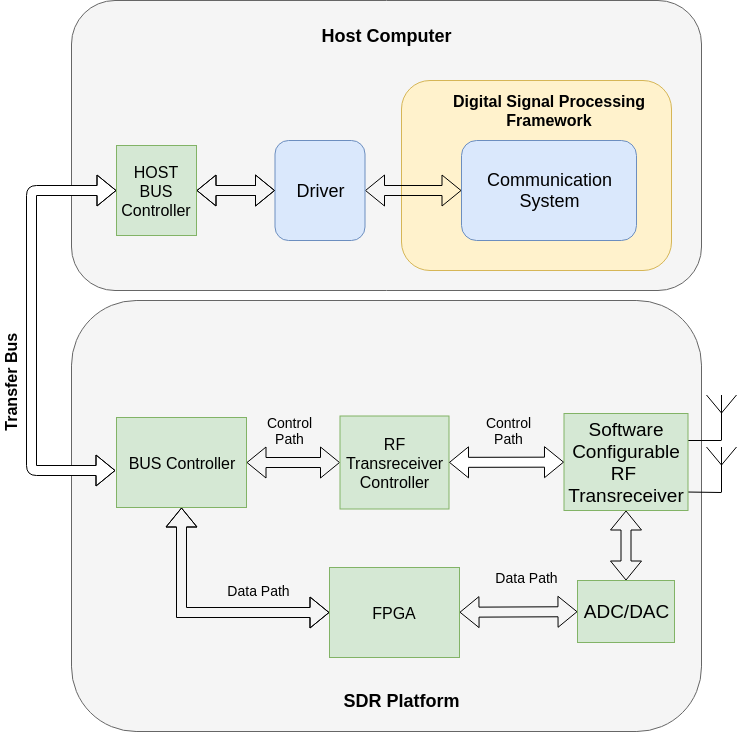
\includegraphics[width=\textwidth]{Figure/Host_Phy.png}
\caption{Host-PHY \cite{nychis_enabling_nodate} \ac{sdr} architecture.}
\end{figure}

\subsection{GNU Radio}

\section{State of the Art}
\section{Base System and Tools}
 
\subsection{LimeSDR-USB}
The LimeSDR-USB uses a USB 3.0 interface for communicating with the host computer. It supports MIMO operations with 2 RX and TX channels operating simultaneously. The maximum sampling rate supported by the ADC and DAC of LMS7002M is 160 Mhz, but the USB 3.0 restricts it to 61.44 MSPS when all the RX and TX channels are used simultaneously.

\subsubsection{LimeSDR USB dataflow.}
\begin{figure}[h!]
\centering
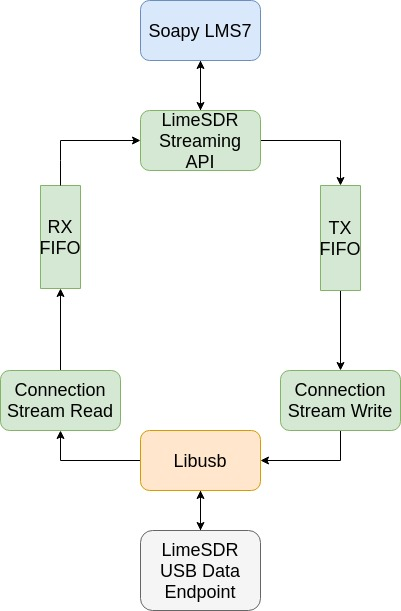
\includegraphics[scale=0.6]{Figure/Software_Architecture.jpg}
\caption{LimeSDR USB software architecture}
\end{figure}

\begin{itemize}
\item{\textit{TX Data Path:} Stream data from GNURadio is passed through Soapy drivers to the LimeSDR Streaming API. The API unwraps the data and the control flags and pushes it to the TX-FIFO. It also does the necessary data representation translation depending on the data format of the streamed data. For example, in case of complex data, it changes 32 bit I and Q value representation of GNU Radio to 16 bit I and Q values representation.  The values are pushed to the respective TX stream channel buffers(TXFIFO). The connection stream initializes the TX buffers and fills them with data from the TXFIFO. The Write function structures the data into FPGA data packet structure((Figure \ref{fpga_packet})) and combines multiple such packets into predefined batch size(initially 4). The buffer is processed by libusb to create bulk transfer packet and finally streamed to output data endpoint.}

\item{\textit{RX Data Path: } The USB data is continuously streamed from the LimeSDR to the Connection stream buffers through libusb. The Read function waits for data to be available from a usb context for the endpoint it is listening to, then it transfer data from the endpoint, parses the FPGA packets (Figure \ref{fpga_packet}) to collect the data and pushes them to the RXFIFO. If the rx stream is configured to have particular receive time, it checks if that condition is satisfied. The LimeSDR streaming API collects the data from the RXFIFO and does the necessary data interpretation translation (reverse translation to the TX Data Path), finally streams the data to GNURadio. }
\end{itemize}

\subsubsection{LimeSDR USB packets and endpoints}
LimeSDR uses four different endpoints for USB data transfer, these endpoints as Data Endpoint and Control Endpoint for both input and output directions. The control endpoints are used for configuring and retrieving data from the LMS7002M and NIOS Core on the FPGA. Data packets are used for the streaming data. 
\begin{table}[h!]
\centering
\begin{tabular}{|c|c|}
\hline
Endpoint No. & Function\\
\hline
0x01 & Stream Data Output\\
0x81 & Stream Data Input\\
0x0F & Control Data Output\\
0x8F & Control Data Input\\
\hline
\end{tabular}
\caption{LimeSDR USB transfer endpoints}
\end{table}
It uses two different packet structures for the LMS7002M Control Packets and the Stream Data Packets. Depending on the control command, different number of bytes are packed into one data element and the maximum number of blocks in a single packet is defined. One LMS64C protocol packet (Figure \ref{lms_packet}) is maximum 64 bytes, if the data to be sent is larger than that then the data field is segmented into several packets. The block count gives the number of data element in a single packet. The FPGA contains 4080 bytes of data along with 8 bytes of counter data that can be used for timestamp on the TX packets. The Lime driver uses synchronous bulk transfer for LMS Control packets and asynchronous bulk transfers for the FPGA packets.
\begin{figure}[h!]
\centering
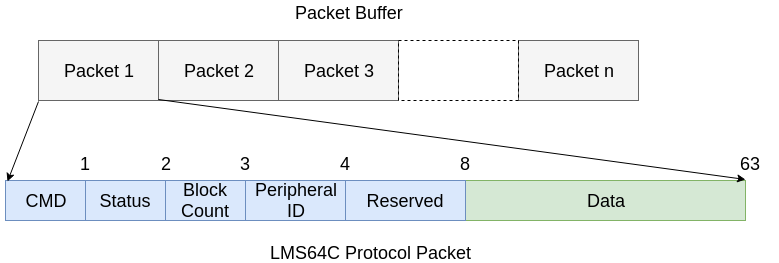
\includegraphics[width=\textwidth]{Figure/LMS64C_Packet.png}
\caption{LMS Control Packet Structure}
\label{lms_packet}
\end{figure}

\begin{figure}[h!]
\centering
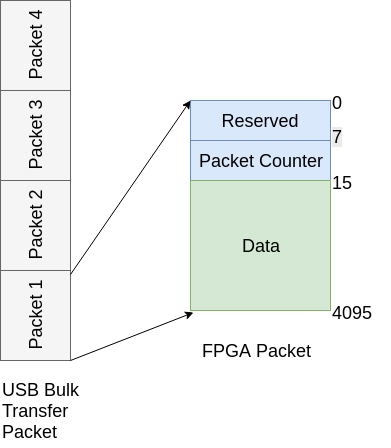
\includegraphics[scale=0.6]{Figure/FPGA_Packet.png}
\caption{FPGA Packet Structure}
\label{fpga_packet}
\end{figure}




\subsection{USBMon}
It is kernel facility provided to collect I/O traces on the USB Bus\cite{_usbmon}. USBMon reports the requests made to and by the USB Host Controller Drivers(HCD). It provides two kinds of API's : binary and character. The binary API is accessed by character devices located in the /dev namespace. The character API provides human readability and uniform format for the traces.The kernel data from the USBMon text data is made available to the userspace using debugfs\cite{_debugfs} utility.

\begin{figure}[h!]
\centering
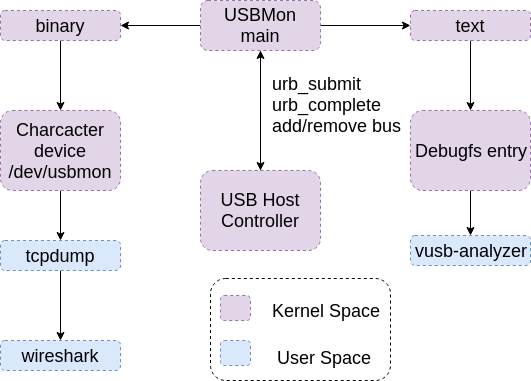
\includegraphics[width=\textwidth]{Figure/USBMon.png}
\caption{USBMon Architecture(Adapted from \cite{basak_usb_2018}).}
\end{figure}

\subsubsection{Text Data Format}
\begin{table}
\centering
\begin{tabular}{|c|c|c|c|c|}
\hline
URB Tag & Timestamp & Event Type & Address & URB Status\\
\hline
ffff8fbdbbae4000 & 2942307806 & S & Bo:3:008:15 & -115\\ 
\hline
\end{tabular}
\begin{tabular}{|c|c|c|}
\hline
Data Length & Data Tag & Data\\
\hline
64 & = & 21000100 00000000 002a0484 00000000 000000\\
\hline
\end{tabular}
\caption{Text USB Trace Example.}
\end{table}

\begin{itemize}
\item {\textit{URB Tag:} URB Identification number, it is usually the in kernel adress of the URB structure.}
\item{\textit{Timestamp:} The timestamp for the URB event at the HCD in microseconds. It is measured by the usbmon main utility using \textit{gettimeofday()} function of \textit{time.h}.}
\item{\textit{Event Type:} It specifies the event type of the HCD event. S - Submission C -Complete E - submission error.}
\item{\textit{Address: } It consists of four fields separated by colons. The URB type and direction, bus number, device number, endpoint number. The URB type and direction specifies the type of USB transfer(can be both synchronous and asynchronous).\\
\begin{table}[h!]
\centering
\begin{tabular}{|c|c|c|}
\hline
Bi & Bo & Bulk Input and Output.\\
Ci & Co & Control Input and Output.\\
Ii & Io & Interrupt Input and Output.\\
Zi & Zo & Isochronous Input and Output.\\
\hline
\end{tabular}
\caption{URB Type and Direction.}
\end{table}\\
The USB device transfers data through a pipe to a memory buffer on the host and endpoint on the device. The type of data transfer depends on the endpoint and the requirements of the function. The transfer types are as follows\cite{_usb_data_transfer}:

\begin{itemize}
\item{\textbf{Control Transfers:} It is mainly used for configuration, command and status operations.}
\item{\textbf{Bulk Transfers:} Bulk Transfer are used for bulky,non-periodic non time-sensitive burst transmissions.}
\item{\textbf{Interrupt Transfers:} It is used for mainly sending small amounts of data infrequently or asynchronously.}
\item{\textbf{Isochronous Transfers:} Isochronous transfers are mainly used for periodic, continuous streams of time sensitive data.} 
\end{itemize}
USB endpoint as explained by \cite{_usb_endpoint} , refers to the buffers on the USB device. The host computer irrespective of the host operating system can communicate by reading and writing to these buffers. They can be data endpoints and control endpoints.Data endpoints are used for transferring data whereas the control endpoint is used for configuration and device specific control.
}

\item{\textit{Data Length:} For urb\_submit it gives the requested data length and for callbacks it is the actual data length.}

\item{\textit{Data tag:} If this field is '=' then data words are present.}

\item{\textit{Data:} The data words contains in the USB transfer packet.}
\end{itemize}

\subsubsection{Raw Binary}
The overall data format is same as the text data, the data is available in raw binary by accessing character devices at /dev/usbmonX. The data can be read by using \textit{read} with \textit{ioctl} or by mapping the buffer using \textit{mmap}. The usbmon events are buffered in the following format:

\begingroup
\centering\scriptsize\begin{lstlisting}
struct usbmon_packet {
	u64 id;			/*  0: URB ID - from submission to callback */
	unsigned char type;	/*  8: Same as text; extensible. */
	unsigned char xfer_type; /*    ISO (0), Intr, Control, Bulk (3) */
	unsigned char epnum;	/*     Endpoint number and transfer direction */
	unsigned char devnum;	/*     Device address */
	u16 busnum;		/* 12: Bus number */
	char flag_setup;	/* 14: Same as text */
	char flag_data;		/* 15: Same as text; Binary zero is OK. */
	s64 ts_sec;		/* 16: gettimeofday */
	s32 ts_usec;		/* 24: gettimeofday */
	int status;		/* 28: */
	unsigned int length;	/* 32: Length of data (submitted or actual) */
	unsigned int len_cap;	/* 36: Delivered length */
	union {			/* 40: */
		unsigned char setup[SETUP_LEN];	/* Only for Control S-type */
		struct iso_rec {		/* Only for ISO */
			int error_count;
			int numdesc;
		} iso;
	} s;
	int interval;		/* 48: Only for Interrupt and ISO */
	int start_frame;	/* 52: For ISO */
	unsigned int xfer_flags; /* 56: copy of URB's transfer_flags */
	unsigned int ndesc;	/* 60: Actual number of ISO descriptors */
};	
\end{lstlisting}
\endgroup


\subsection{pidstat}
\subsection{802.15.4}